%%% Preamble
  \documentclass[paper=a4, fontsize=11pt]{scrartcl}
  \usepackage[T1]{fontenc}
  \usepackage{fourier}

  \usepackage[english]{babel}
  \usepackage[protrusion=true,expansion=true]{microtype}
  \usepackage{amsmath,amsfonts,amsthm}
  \usepackage[pdftex]{graphicx}
  \usepackage{url}
  \usepackage{setspace}
  \usepackage{vmargin}
  \setmarginsrb   {1.25in}  % left margin
                  { 0.6in}  % top margin
                  { 1.0in}  % right margin
                  { 0.8in}  % bottom margin
                  {  20pt}  % head height
                  {0.25in}  % head sep
                  {   9pt}  % foot height
                  { 0.3in}  % foot sep

  \usepackage{sectsty}
  \allsectionsfont{\centering \normalfont\scshape}

  % Bibliography
  \usepackage{natbib}
  \bibliographystyle{aer}



  %%% Custom headers/footers (fancyhdr package)
  \usepackage{fancyhdr}
  \fancyhead[L]{\small Spencer Lyon: Superconductor Report}
  \fancyhead[R]{\thepage}
  \fancyfoot{} % no footer
  \renewcommand{\headrulewidth}{.5pt}
  \renewcommand{\footrulewidth}{.5pt}
  \setlength{\headheight}{13.6pt}


  %%% Equation and float numbering
  \numberwithin{equation}{section}
  \numberwithin{figure}{section}
  \numberwithin{table}{section}

  %%% Maketitle metadata
  \newcommand{\horrule}[1]{\rule{\linewidth}{#1}}     % Horizontal rule

  \title{
    \vspace{-.3in}
    \usefont{OT1}{bch}{b}{n}
    \normalfont \normalsize \textsc{Physics 240} \\ [25pt]
    \horrule{0.5pt} \\[0.4cm]
    \huge Resistance vs. Temperature of a phase 2223 BSCCO Superconductor \\
    \horrule{2pt} \\[0.5cm]
  }

  \author{
    Spencer Lyon
    \thanks{I thank Chuck for building circuits, taking measurements, and being cool.}
  }

  \date{
  \normalfont \normalsize
  \today \\[-4pt] \normalsize
  }


%%% Begin document
\begin{document}

  \begin{titlepage}
      \pagestyle{empty}
      \maketitle

      \begin{abstract}
            \begin{center}
            \small{
                  In this paper I analyze the properties of a Pb-doped BSCCO superconductor ($Bi_{2-x}Pb_xSr_2Ca_{y-1}Cu_yO_{\delta}$). Specifically I examined how the the resistivity of the superconductor varies with respect to temperature. To measure the temperature I coupled the superconductor with a diode and fit a linear model to the temperature response of the diode. I found that the transition temperature for the superconductor is about $110^{\circ} C$. The transition is fairly clear and looks much like a step function. I also found that the superconductor behaves more like a metal than a semiconductor after it crosses the critical temperature.
            }
            \end{center}
      \end{abstract}
  \end{titlepage}

  \pagestyle{fancyplain}
  \setcounter{page}{1}

  \section{Introduction}
      \setstretch{2}

      Superconductivity occurs when a substance exhibits identically zero electrical resistance. Superconductivity was discovered in 1911 and has been an active part of physics research ever since. Superconductors are valuable because of the many ways in which they can be applied. A few examples of applications for superconductors are powerful electro magnets, mass spectrometers, magnets used in particle accelerators, power storage, and quantum computing.For a material to superconduct, it must be cooled below a transition or critical temperature. This temperature is different for all superconductors, and the focus of this research was to find the critical temperature for the $Bi_{2-x}Pb_xSr_2Ca_{y-1}Cu_yO_{\delta}$ (BSCCO) superconductor.

      The earliest experiments with superconductors having high critical temperatures were carried out in the late 1980's. Groups from all over the world were excited about the possibilities associated with high-temperature superconductivity. In 1987, physicists found substances that exhibited superconductivity in at $90K$ in a $(Ba-Y-Cu-O)$ system \citep{Ashburn:1987}. Shortly thereafter there were flood of studies analyzing the behavior and finding the critical temperature of the BSCCO superconductors under various conditions.

      Specifically, \citet{yanagisawa:1988} found that by a partial substitution of $Pb$ for $Bi$ in the BSCCO compound ($Pb$-doping), they came up with a compound that had a current-dependent transition temperature ($T_c$) somewhere in the range of $102-110K$. They found that as they increased the current through the superconductor from $0.2 mA$ to $100 mA$, $T_c$ moved from $108$ to $110 K$.

      Just one year later \citet{LeePark:1989} expounded further on the behavior of the BSCCO superconductor and found that there were two phases at which the BSCCO compound would transition. They named the two temperatures low-$T_c$ ($80K$) and high-$T_c$ ($110K$). For the 2223-phase BSCCO superconductor (the one used in my experiment), they ultimately ended up with superconduction at a temperature of $108K$.

      Contemporary experiments were done in California during 1989 that found that BSCCO compounds have at least three different phases transition temperatures \citep{Green:1989}. Of the three compounds studied, \citet{Green:1989} determined that the 2223 phase was the most stable. The transition temperature they reported was $111.5K$.

      Research on bismuth ($Bi$) based superconductors didn't stop in the 80's. \citet{anis:2009} examined the macroscopic properties of Pb-doped BSCCO superconductors. Among the things that they studied were dc resistivity, susceptibility, thermal transport, electrothermal conductivity and thermoelectric properties as a function of temperature. Their ultimate findings on resistivity match the early studies from the 1980's with $T_c \approx 110K \pm 1K$.

      My research follows the  basic structure of the articles mentioned above in that I examine the thermal resistivity response of a BSCCO superconductor. To carry out the experiment I needed an accurate thermometer, LabView VI's to measure resistance and temperature, and liquid nitrogen to get the system cooled below the transition temperature.

  \section{Experimental Methods and Materials}

      The process by which I gathered data for this experiment can be broken down into 2 logical categories: preparation and collection. We will look at each of these processes in more detail below.

      \subsection{Preparation}

            Much of the preparation of the superconductor was done by the BYU faculty. In order to measure the temperature and the resistance, the superconductor needed to be held at the same temperature as something I could easily measure the temperature of. A 1N4148 diode has the remarkable property that its resistance response to temperature is extremely close to linear. Knowing this, the faculty attached one of these diodes to the BSCCO superconductor as shown in Figure ~\ref{fig:scDiode}.

            \begin{figure}[h]
                  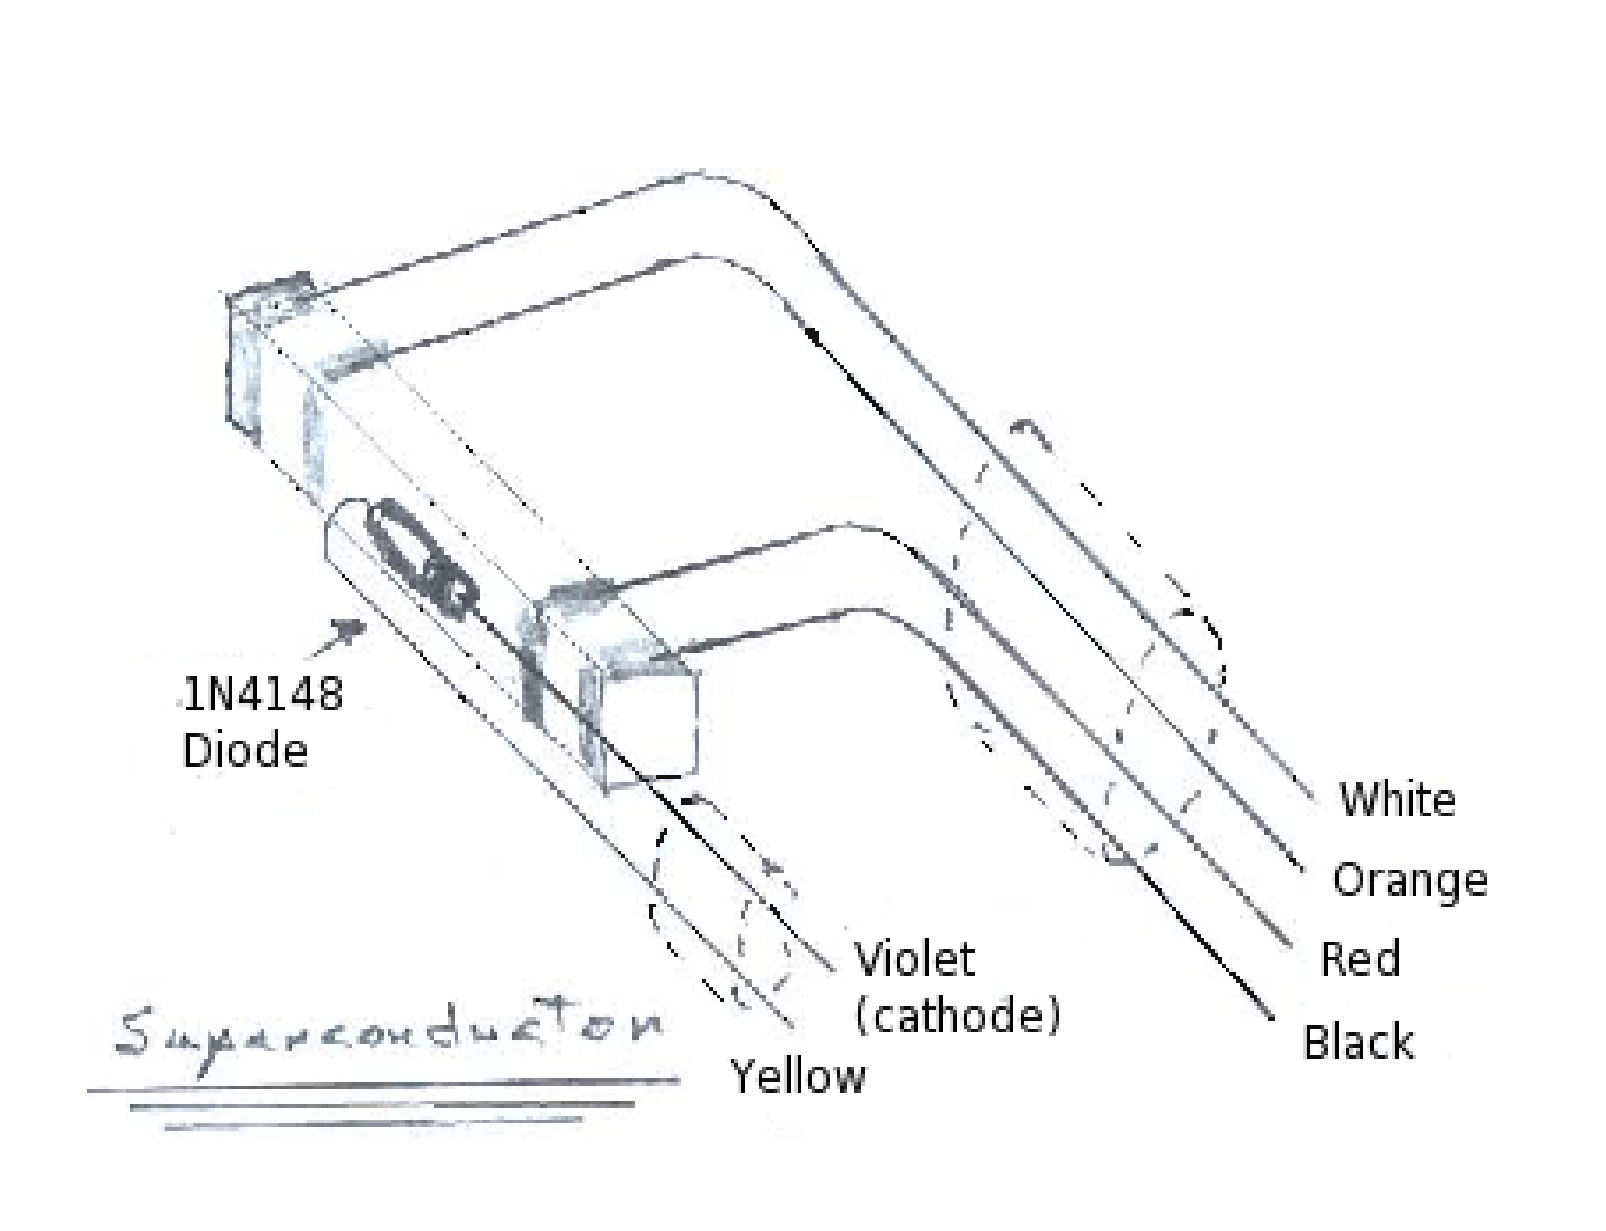
\includegraphics[width=0.9\textwidth]{Figures/SuperconductorDrawing.eps}
                  \caption{Connection diagram of superconductor and diode}
                  \label{fig:scDiode}
            \end{figure}

            Another important part of the preparation phase was to calibrate the diode. To do this

      \subsection{Collection}

            fd

  \section{Results}

      put some results here

  \section{Discussion of Results}

      discuss those results

  \clearpage
  \pagestyle{empty}
  \bibliography{scReport}

  %%% End document

\end{document}
